\documentclass{article}
\usepackage[none]{hyphenat}
\DeclareUnicodeCharacter{2212}{\ensuremath{-}}
\usepackage{graphicx}

\title{Assignment 4}
\date{}

\begin{document}

\maketitle

\section*{CH22B106}

\textbf{Name: }Sukriti Choudhary

\noindent\textbf{Github user-id: }Sukriti-c

\subsection*{Euler's Identity}

Leonhard Euler was an $18^{th}$ century Swiss-born mathematician who developed many concepts that are integral to modern mathematics. One of his important contributions was the
\textbf{Euler's identity}

$$ e^{i\pi} + 1 = 0 $$ 

\noindent Euler’s identity is often regarded as the “most beautiful mathematics equation” because of its simplicity and ability to show the relationship between five essential constants of mathematics~\cite{stipp2017most}. No other equation expresses the relationship of so many constants across various mathematical fields in such a simple way. The constants are:

\begin{itemize}

\item The number 0, the additive identity.
\item The number 1, the multiplicative identity.
\item The number $\pi$ ($\pi$ = 3.1415...), the fundamental circle constant
\item The number e (e = 2.718...), also known as Euler's number, which occurs widely in mathematical analysis
\item The number i, the imaginary unit of the complex numbers
 
\end{itemize}

\subsection*{Trigonometric uses}~\cite{nair2018euler}
\noindent Euler’s identity has several applications within mathematics. It allows standard trigonometric functions to be expressed in terms of exponential functions as 
$ \cos x = \frac{e^{ix} + e^{−ix}}{2} $
and
$ \sin x = \frac{e^{ix} − e^{−ix}}{2i} $
and can be used in verifying the addition and subtraction formulas for sine and cosine.\\

\subsection*{Logarithms of Negative Numbers}~\cite{nair2018euler}
\noindent The unusual idea of finding the logarithm of a negative number became a reality as from the
identity it follows that $\ln$(−1) = i$\pi$.

\subsection*{Complex Numbers Raised to Complex Numbers}~\cite{nair2018euler}
\noindent A remarkable consequence of this identity is that it allows us to compute complex powers of complex numbers which turn out to be real numbers. For
example substituting $x = \frac{\pi}{2}$
in the identity we get $e^{\frac{i\pi}{2}}=i$, now raising this to i we get
$$i^{i} = e^{\frac{-\pi}{2}} \approx 0.2078796$$
These repercussions of Euler’s identity allows us to manipulate complex numbers
and has profound implications in complex number theory.

\subsection*{Conclusion}
\noindent In conclusion, Euler's identity has applications in various fields of theoretical mathematics as well as real world of problem solving. It is a really wonderful expression and to express its beauty, one of the limericks written by Paul Nahin is as follows~\cite{nahin2011dr}: \\

\begin{figure}[h] 
	\begin{center}
		\framebox{
			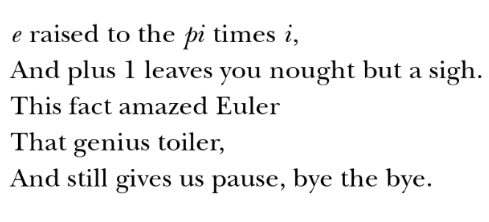
\includegraphics[scale=0.7]{limerick.png} 
		}
	\end{center}
\end{figure}

\bibliography{refs}
\bibliographystyle{alpha}


\end{document}
